\documentclass[]{article}
\usepackage{graphicx}
\usepackage[svgnames]{xcolor} 
\usepackage{fancyhdr}

\usepackage{hyperref}
\usepackage{enumitem}
\usepackage[many]{tcolorbox}
\usepackage{listings }
\usepackage[a4paper, total={6in, 8in}]{geometry}
\usepackage{afterpage}
\usepackage{amssymb}
\usepackage{xepersian}
\usepackage[T1]{fontenc}
\usepackage{tikz}
\usepackage[utf8]{inputenc}
\usepackage{PTSerif} 
\usepackage{seqsplit}

\usepackage{listings}
\usepackage{xcolor}
 
\definecolor{codegreen}{rgb}{0,0.6,0}
\definecolor{codegray}{rgb}{0.5,0.5,0.5}
\definecolor{codepurple}{rgb}{0.58,0,0.82}
\definecolor{backcolour}{rgb}{0.95,0.95,0.92}
 
\NewDocumentCommand{\codeword}{v}{
\texttt{\textcolor{blue}{#1}}
}
\lstset{language=C,keywordstyle={\bfseries \color{blue}}}

\lstdefinestyle{mystyle}{
    backgroundcolor=\color{backcolour},   
    commentstyle=\color{codegreen},
    keywordstyle=\color{magenta},
    numberstyle=\tiny\color{codegray},
    stringstyle=\color{codepurple},
    basicstyle=\ttfamily\normalsize,
    breakatwhitespace=false,         
    breaklines=true,                 
    captionpos=b,                    
    keepspaces=true,                 
    numbers=left,                    
    numbersep=5pt,                  
    showspaces=false,                
    showstringspaces=false,
    showtabs=false,                  
    tabsize=2
}

\lstset{style=mystyle}

\settextfont[BoldFont={XB Zar bold.ttf}]{XB Zar.ttf}




\newcommand{\inputsample}[1]{
    ~\\
    \textbf{ورودی نمونه}
    ~\\
    \begin{tcolorbox}[breakable,boxrule=0pt]
        \begin{latin}
            \large{
                #1
            }
        \end{latin}
    \end{tcolorbox}
}

\newcommand{\outputsample}[1]{
    ~\\
    \textbf{خروجی نمونه}

    \begin{tcolorbox}[breakable,boxrule=0pt]
        \begin{latin}
            \large{
                #1
            }
        \end{latin}
    \end{tcolorbox}
}

%%%%%باکس های طراحی شده برای پاسخ نامه ، میتوانید پاسخ را درون باکس قراردهید
\newtcolorbox[auto counter]{solutionbox}{
freelance,
colback=white,
frame code={},
interior titled code={
  \fill[rounded corners=8pt,orange!30]
    (title.south west) --
    (title.south) -- 
    ([yshift=20pt]title.south) --
    ([yshift=20pt,xshift=4cm]title.south) --
    ([xshift=4cm]title.south) --
    (title.south east) {[sharp corners] --
    ([yshift=-6pt]title.south east) -- 
    ([yshift=-6pt]title.south west) } -- cycle;
  \draw[rounded corners=8pt,gray,line width=1pt]
    (title.west|-frame.south west) --
    (title.south west) --
    (title.south) -- 
    ([yshift=20pt]title.south) --
    ([yshift=20pt,xshift=4cm]title.south) --
    ([xshift=4cm]title.south) --
    (title.south east) --
    (title.east|-frame.south east) --
    cycle;
  \node at ([xshift=2cm,yshift=4pt,anchor=south]title.south) 
    {\Large \textbf{پاسخ}};  
  },
title={\mbox{}},
top=12pt,
fontupper=\sffamily\Large,
oversize=0.5cm,
before={\vskip24pt\par\noindent},
after={\par\vskip12pt}
}
\newtcolorbox[auto counter]{solutionboxC}{
freelance,
colback=white,
frame code={},
interior titled code={
  \fill[rounded corners=8pt,orange!30]
    (title.south west) --
    (title.south) -- 
    ([yshift=20pt]title.south) --
    ([yshift=20pt,xshift=4cm]title.south) --
    ([xshift=4cm]title.south) --
    (title.south east) {[sharp corners] --
    ([yshift=-6pt]title.south east) -- 
    ([yshift=-6pt]title.south west) } -- cycle;
  \draw[rounded corners=8pt,gray,line width=1pt]
    (title.west|-frame.south west) --
    (title.south west) --
    (title.south) -- 
    ([yshift=20pt]title.south) --
    ([yshift=20pt,xshift=4cm]title.south) --
    ([xshift=4cm]title.south) --
    (title.south east) --
    (title.east|-frame.south east) --
    cycle;
  \node at ([xshift=2cm,yshift=4pt,anchor=south]title.south) 
    {\Large \textbf{ پاسخ ادامه}};  
  },
title={\mbox{}},
top=12pt,
fontupper=\sffamily\Large,
oversize=0.5cm,
before={\vskip24pt\par\noindent},
after={\par\vskip12pt}
}

\begin{document}


%%% title pages
\begin{titlepage}
\begin{center}
        
\vspace*{0.7cm}


\includegraphics[width=0.4\textwidth]{sharif1.png}\\
\vspace{0.5cm}
\textbf{ \Huge{\emph درس برنامه‌سازی پیشرفته} }\\
\vspace{0.5cm}
\textbf{ \Large{ تمرین اول} }
\vspace{0.2cm}
       
 
      \large \textbf{دانشکده مهندسی کامپیوتر}\\\vspace{0.2cm}
    \large   دانشگاه صنعتی شریف\\\vspace{0.2cm}
       \large   ﻧﯿﻢ سال دوم 99-98 \\\vspace{0.2cm}
      \noindent\rule[1ex]{\linewidth}{1pt}
    مبحث:\\
    \textbf{{مباحث مقدماتی جاوا}}

    \vspace{0.20cm}

   مهلت ارسال:\\
    \textbf{{19 اسفند}}\\
    \textbf{{ساعت 23:59}}

    \vspace{0.15cm}
ویراستار فنی:\\
    \textbf{{صابر ظفر‌پور و محمّد فراهانی}}
\end{center}
\end{titlepage}
%%% title pages


%%% header of pages
\newpage
\pagestyle{fancy}
\fancyhf{}
\fancyfoot{}
\cfoot{\thepage}
\chead{مباحث مقدماتی جاوا}
\rhead{
\includegraphics[width=0.1\textwidth]{sharif.png}}
\lhead{تمرین ۱ برنامه‌سازی پیشرفته}
%%% header of pages




 \Large \textbf{\\\\
به موارد زیر توجه کنید:}

\begin{itemize}[label=$\ast$]
\item به‌ازای هر سوال در سامانه‌ی کوئرا، یک بخش جداگانه برای بارگذاری برنامه‌ی شما وجود دارد. برنامه‌ی خود با پسوند .java را در بخش مربوط به هر سوال بارگذاری کنید.
\item ورودی و خروجی شما باید عیناً شبیه به نمونه‌های ورودی و خروجی باشد؛ لذا عبارت‌هایی همچون \lr{"Enter your number"} را قبل از گرفتن ورودی نباید چاپ کنید.
\item پس از ارسال فایل مربوط به هر سوال، سامانه‌ی کوئرا به‌صورت لحظه‌ای برنامه‌ی شما را داوری کرده و نمره‌ی آن سوال را به شما اعلام می‌کند که در صورت کم بودن نمره‌تان، می‌توانید آن را تصحیح کرده و دوباره ارسال کنید.
\item هم‌فکری و هم‌کاری در پاسخ به تمرینات اشکالی ندارد و حتی توصیه نیز می‌شود؛ ولی پاسخ ارسالی شما باید حتما توسط خود شما نوشته شده‌باشد. در صورت هم‌فکری در مورد یک سوال، نام افراد دیگر را به‌صورت کامنت در ابتدای کد هر سوال بنویسید.  این نکته رو در نظر بگیرید که هم‌فکری تنها مربوط به بخش ایده سوال هست نه پیاده‌سازی آن و در صورت محرز شدن تقلب برای فرد خاطی بدون مسامحه \emph{ منفی نمره تمرین}
منظور می‌گردد. 
\item شما می‌توانید تمامی سوالات و ابهامات خود را در سایت کوئرا در بخش مشخص‌شده برای این تمرین بپرسید.
\item به‌ازای هر روز تاخیر در ارسال پاسخ هر سوال، 30 درصد از نمره‌ی کسب‌شده‌ی شما در آن سوال کم می‌شود. به عنوان مثال اگر پاسخ یک سوال را با دو روز تاخیر ارسال کنید، فقط 40 درصد از نمره‌ای که برای آن سوال گرفته‌اید برای شما لحاظ خواهد شد.
\item در کل شما می‌توانید سه روز تاخیر بدون کسر نمره داشته باشد.
\item به ازای هر‌روز ارسال زود‌تر تمرین به شرط کامل بودن، 5\% نمره اضافه به شما تعلق می‌گیرد. سقف تعداد روز‌هایی که  برای این موضوع محاسبه می‌شود چهار است یعنی در صورت ارسال زود‌تر از چهار روز فقط 20\% نمره اضافه به شما تعلق می‌گیرد. 
\item مهلت ارسال تمرین تا ساعت 23:59 روز 19 اسفند 1398 است.
\end{itemize}



\newpage
\section{طراحی نماد}
هاشم که به تازگی رئیس سازمان لیگ شده است، به فکر تغییر نمادهای تیم های حاضر در لیگ افتاده است! او که فکر می‌کند تیم های حاضر در لیگ بسیار قدرتمند و پرافتخار هستند ، معتقد است باید نمادی برازنده افتخارات و قدرتشان داشته باشند! برای همین تمام فکر خود را به کار می‌گیرد (!) و تصمیم می‌گیرد که نمادی با طرح ستاره برای تیم‌ها طراحی کند! اما این طرح ستاره به گونه‌ای است که ستاره­‌ها به شکل یک نوار، حاشیه‌ی یک لوزی با قطرهای برابر را پر می‌کنند. قطر لوزی 
\lr{(2n + 1)}
، برابر سال‌هایی است که یک تیم در لیگ حضور داشته‌است و پهنای این نوار بسته به افتخاراتی که آن تیم تا به حال کسب کرده عددی متغیر (k) است. حال که هاشم این فکر استثنایی به ذهنش رسیده تنها مشکلش این است که چگونه این نمادها را برای تیم‌ها آماده کند. برنامه‌ای بنویسید که طرح مورد نظر هاشم را با گرفتن n و k چاپ کند.\\

\textbf{ورودی}
\\\\
ابتدا n و سپس k با یک فاصله در ورودی داده می‌شود. ( n و k اعدادی طبیعی‌اند.)\\

\textbf{خروجی}
\\\\
در خروجی ستاره‌ها متناسب با ورودی چاپ می‌شوند.
\\
\newpage
\inputsample{
1 4
}

\outputsample{
\texttt{\char32}\texttt{\char32}\texttt{\char32}\texttt{\char32}*\\
\texttt{\char32}\texttt{\char32}\texttt{\char32}*\texttt{\char32}*\\
\texttt{\char32}\texttt{\char32}*\texttt{\char32}\texttt{\char32}\texttt{\char32}*\\
\texttt{\char32}*\texttt{\char32}\texttt{\char32}\texttt{\char32}\texttt{\char32}\texttt{\char32}*\\
*\texttt{\char32}\texttt{\char32}\texttt{\char32}\texttt{\char32}\texttt{\char32}\texttt{\char32}\texttt{\char32}*\\
\texttt{\char32}*\texttt{\char32}\texttt{\char32}\texttt{\char32}\texttt{\char32}\texttt{\char32}*\\ 
\texttt{\char32}\texttt{\char32}*\texttt{\char32}\texttt{\char32}\texttt{\char32}*\\
\texttt{\char32}\texttt{\char32}\texttt{\char32}*\texttt{\char32}*\\
\texttt{\char32}\texttt{\char32}\texttt{\char32}\texttt{\char32}*
}
\newpage
\inputsample{
3 10
}

\outputsample{
\texttt{\char32}\texttt{\char32}\texttt{\char32}\texttt{\char32}\texttt{\char32}\texttt{\char32}\texttt{\char32}\texttt{\char32}\texttt{\char32}\texttt{\char32}*\\
\texttt{\char32}\texttt{\char32}\texttt{\char32}\texttt{\char32}\texttt{\char32}\texttt{\char32}\texttt{\char32}\texttt{\char32}\texttt{\char32}***\\
\texttt{\char32}\texttt{\char32}\texttt{\char32}\texttt{\char32}\texttt{\char32}\texttt{\char32}\texttt{\char32}\texttt{\char32}*****\\
\texttt{\char32}\texttt{\char32}\texttt{\char32}\texttt{\char32}\texttt{\char32}\texttt{\char32}\texttt{\char32}***\texttt{\char32}***\\
\texttt{\char32}\texttt{\char32}\texttt{\char32}\texttt{\char32}\texttt{\char32}\texttt{\char32}***\texttt{\char32}\texttt{\char32}\texttt{\char32}***\\
\texttt{\char32}\texttt{\char32}\texttt{\char32}\texttt{\char32}\texttt{\char32}***\texttt{\char32}\texttt{\char32}\texttt{\char32}\texttt{\char32}\texttt{\char32}***\\
\texttt{\char32}\texttt{\char32}\texttt{\char32}\texttt{\char32}***\texttt{\char32}\texttt{\char32}\texttt{\char32}\texttt{\char32}\texttt{\char32}\texttt{\char32}\texttt{\char32}***\\
\texttt{\char32}\texttt{\char32}\texttt{\char32}***\texttt{\char32}\texttt{\char32}\texttt{\char32}\texttt{\char32}\texttt{\char32}\texttt{\char32}\texttt{\char32}\texttt{\char32}\texttt{\char32}***\\
\texttt{\char32}\texttt{\char32}***\texttt{\char32}\texttt{\char32}\texttt{\char32}\texttt{\char32}\texttt{\char32}\texttt{\char32}\texttt{\char32}\texttt{\char32}\texttt{\char32}\texttt{\char32}\texttt{\char32}***\\
\texttt{\char32}***\texttt{\char32}\texttt{\char32}\texttt{\char32}\texttt{\char32}\texttt{\char32}\texttt{\char32}\texttt{\char32}\texttt{\char32}\texttt{\char32}\texttt{\char32}\texttt{\char32}\texttt{\char32}\texttt{\char32}***\\
***\texttt{\char32}\texttt{\char32}\texttt{\char32}\texttt{\char32}\texttt{\char32}\texttt{\char32}\texttt{\char32}\texttt{\char32}\texttt{\char32}\texttt{\char32}\texttt{\char32}\texttt{\char32}\texttt{\char32}\texttt{\char32}\texttt{\char32}***\\
\texttt{\char32}***\texttt{\char32}\texttt{\char32}\texttt{\char32}\texttt{\char32}\texttt{\char32}\texttt{\char32}\texttt{\char32}\texttt{\char32}\texttt{\char32}\texttt{\char32}\texttt{\char32}\texttt{\char32}\texttt{\char32}***\\
\texttt{\char32}\texttt{\char32}***\texttt{\char32}\texttt{\char32}\texttt{\char32}\texttt{\char32}\texttt{\char32}\texttt{\char32}\texttt{\char32}\texttt{\char32}\texttt{\char32}\texttt{\char32}\texttt{\char32}***\\
\texttt{\char32}\texttt{\char32}\texttt{\char32}***\texttt{\char32}\texttt{\char32}\texttt{\char32}\texttt{\char32}\texttt{\char32}\texttt{\char32}\texttt{\char32}\texttt{\char32}\texttt{\char32}***\\
\texttt{\char32}\texttt{\char32}\texttt{\char32}\texttt{\char32}***\texttt{\char32}\texttt{\char32}\texttt{\char32}\texttt{\char32}\texttt{\char32}\texttt{\char32}\texttt{\char32}***\\
\texttt{\char32}\texttt{\char32}\texttt{\char32}\texttt{\char32}\texttt{\char32}***\texttt{\char32}\texttt{\char32}\texttt{\char32}\texttt{\char32}\texttt{\char32}***\\
\texttt{\char32}\texttt{\char32}\texttt{\char32}\texttt{\char32}\texttt{\char32}\texttt{\char32}***\texttt{\char32}\texttt{\char32}\texttt{\char32}***\\
\texttt{\char32}\texttt{\char32}\texttt{\char32}\texttt{\char32}\texttt{\char32}\texttt{\char32}\texttt{\char32}***\texttt{\char32}***\\
\texttt{\char32}\texttt{\char32}\texttt{\char32}\texttt{\char32}\texttt{\char32}\texttt{\char32}\texttt{\char32}\texttt{\char32}*****\\
\texttt{\char32}\texttt{\char32}\texttt{\char32}\texttt{\char32}\texttt{\char32}\texttt{\char32}\texttt{\char32}\texttt{\char32}\texttt{\char32}***\\
\texttt{\char32}\texttt{\char32}\texttt{\char32}\texttt{\char32}\texttt{\char32}\texttt{\char32}\texttt{\char32}\texttt{\char32}\texttt{\char32}\texttt{\char32}*
}

\newpage


\section{کمیتهٔ انضباطی}
عرفان به تازگی رئیس کمیتهٔ انضباطی فدراسیون فوتبال شده و می‌خواهد قبل از شروع لیگ تخلفات تیم‌های متخلف را شناسایی کرده و از شرکت آنها در لیگ ممانعت به عمل آورد! لیگ تا ۲ هفتهٔ دیگر شروع می‌شود و مهلت نقل و انتقالات به تازگی به پایان رسیده. اسامی بازیکان مجاز جهت شرکت در لیگ به همراه اسامی تیم‌ها و بازیکنان هر تیم به سازمان لیگ داده شده است.\\
عرفان که به تنهایی نمی‌تواند در بین همهٔ اسامی تخلفات را پیدا کند از شما می‌خواهد که برنامه‌ای بنویسید که تخلفات تیم‌های مختلف را شناسایی کرده و گزارش کنید.\\\\
موارد زیر درصورت وقوع به عوان تخلف شناخته خواهند شد:
\begin{itemize}[label=$\ast$]
\item 	در بین اسامی بازیکنان یک تیم بازیکنی وجود داشته باشد که نام آن در لیست بازیکنان مجاز جهت شرکت در لیگ نیست. در این صورت آن تیم به عنوان متخلف شناخته خواهد شد.
\item	 اسم یک بازیکن در چند تیم وجود داشته باشد (بازیکن با چند تیم قرارداد بسته باشد)  در این صورت تمامی تیم‌هایی که بازیکن با آنها قرارداد بسته تخلف کرده اند.\\
\end{itemize}

\textbf{ورودی}\\\\
در خط اول دو عدد n و m داده می‌شوند که به ترتیب تعداد بازیکن‌ها و تعداد تیم‌ها هستند.\\
در n خط بعدی در هر خط نام یک بازیکن داده می‌شود که به صورت یک string و شامل حروف کوچک انگلیسی و فاصله (space) است.\\
سپس در خطوط بعدی به ازای تیم i ام در خط اول نام تیم i ام داده می‌شود که شامل حروف کوچک انگلیسی و space است و خط بعدی عدد a(i) که تعداد بازیکنان تیم i ام است داده می‌شود. سپس در a(i) خط بعدی بازیکنان تیم i ام داده می‌شود\\

\textbf{خروجی}
\\\\
در خروجی باید نام تیم‌های متخلف را به ترتیب حروف الفبا چاپ کنید.\\
\inputsample{
136 6\\
dani carvajal\\
eder militao\\
sergio ramos\\
raphael varane\\
nacho\\
eden hazard\\
toni kroos\\
karim benzema\\
luka modric\\
gareth bale\\
marcelo\\
thibaut courtois\\
casemiro\\
federico valverde\\
james rodriguez\\
lucas vazquez\\
luka jovic\\
marco asensio\\
brahim diaz\\
isco\\
ferland mendy\\
mariano\\
vinicius junior\\
rodrygo\\
marc andre ter stegen\\
nelson semedo\\
gerard pique\\
ivan rakitic\\
sergio busquets\\
arthur\\
luis suarez\\
lionel messi\\
ousmane dembele\\
neto\\
clement lenglet\\
antoine griezmann\\
jordi alba\\
sergi roberto\\
frenkie de jong\\
arturo vidal\\
samuel umtiti\\
junior firpo\\
tomas vaclik\\
sergi gomez\\
lucas ocampos\\
daniel carrico\\
rony lopes\\
nolito\\
ever banega\\
munir\\
jules kounde\\
bono\\
suso\\
youssef en nesyri\\
jesus navas\\
nemanja gudelj\\
sergio escudero\\
luuk de jong\\
diego carlos\\
oliver torres\\
franco vazquez\\
sergio reguilon\\
joan jordan\\
fernando\\
javi diaz\\
antonio adan\\
jose gimenez\\
santiago arias\\
thomas partey\\
koke\\
aoao felix\\
saul\\
alvaro morata\\
angel correa\\
thomas lemar\\
renan lodi\\
jan oblak\\
marcos llorente\\
stefan savic\\
hector herrera\\
ivan saponjic\\
felipe\\
diego costa\\
vitolo\\
yannick carrasco\\
mario hermoso\\
kieran trippier\\
sime vrsaljko\\
alex remiro\\
joseba zaldua\\
diego llorente\\
asier illarramendi\\
igor zubeldia\\
aritz elustondo\\
portu\\
mikel merino\\
willian jose\\
mikel oyarzabal\\
adnan januzaj\\
aihen munoz\\
miguel angel moya\\
ander guevara\\
david zurutuza\\
andoni gorosabel\\
alexander isak\\
nacho monreal\\
martin odegaard\\
ander barrenetxea\\
luca sangalli\\
robin le normand\\
andoni zubiaurre\\
jaume domenech\\
thierry correia\\
jaume costa\\
eliaquim mangala\\
gabriel paulista\\
geoffrey kondogbia\\
goncalo guedes\\
carlos soler\\
kevin gameiro\\
dani parejo\\
denis cheryshev\\
mouctar diakhaby\\
jasper cillessen\\
jose gaya\\
manu vallejo\\
lee kang in\\
francis coquelin\\
daniel wass\\
rodrigo\\
ferran torres\\
cristiano piccini\\
maxi gomez\\
ruben sobrino\\
ezequiel garay\\
alessandro florenzi\\
real madrid\\
25\\
dani carvajal\\
eder militao\\
sergio ramos\\
raphael varane\\
nacho\\
eden hazard\\
toni kroos\\
karim benzema\\
luka modric\\
gareth bale\\
marcelo\\
thibaut courtois\\
casemiro\\
federico valverde\\
james rodriguez\\
lucas vazquez\\
luka jovic\\
marco asensio\\
brahim diaz\\
martin odegaard\\
isco\\
ferland mendy\\
mariano\\
vinicius junior\\
rodrygo\\
barcelona\\
18\\
marc andre ter stegen\\
nelson semedo\\
gerard pique\\
ivan rakitic\\
sergio busquets\\
arthur\\
luis suarez\\
lionel messi\\
ousmane dembele\\
neto\\
clement lenglet\\
antoine griezmann\\
jordi alba\\
sergi roberto\\
frenkie de jong\\
arturo vidal\\
samuel umtiti\\
junior firpo\\
sevilla\\
23\\
tomas vaclik\\
sergi gomez\\
lucas ocampos\\
daniel carrico\\
rony lopes\\
nolito\\
ever banega\\
munir\\
jules kounde\\
bono\\
suso\\
youssef en nesyri\\
jesus navas\\
nemanja gudelj\\
sergio escudero\\
luuk de jong\\
diego carlos\\
oliver torres\\
franco vazquez\\
sergio reguilon\\
joan jordan\\
fernando\\
javi diaz\\
atletico madrid\\
23\\
antonio adan\\
jose gimenez\\
santiago arias\\
thomas partey\\
koke\\
aoao felix\\
saul\\
alvaro morata\\
angel correa\\
thomas lemar\\
renan lodi\\
jan oblak\\
marcos llorente\\
stefan savic\\
hector herrera\\
ivan saponjic\\
felipe\\
diego costa\\
vitolo\\
yannick carrasco\\
mario hermoso\\
kieran trippier\\
sime vrsaljko\\
real sociedad\\
23\\
alex remiro\\
joseba zaldua\\
diego llorente\\
asier illarramendi\\
igor zubeldia\\
aritz elustondo\\
portu\\
mikel merino\\
willian jose\\
mikel oyarzabal\\
adnan januzaj\\
aihen munoz\\
miguel angel moya\\
ander guevara\\
david zurutuza\\
andoni gorosabel\\
alexander isak\\
nacho monreal\\
martin odegaard\\
ander barrenetxea\\
luca sangalli\\
robin le normand\\
andoni zubiaurre\\
valencia\\
25\\
jaume domenech\\
thierry correia\\
jaume costa\\
eliaquim mangala\\
gabriel paulista\\
geoffrey kondogbia\\
goncalo guedes\\
carlos soler\\
kevin gameiro\\
dani parejo\\
denis cheryshev\\
mouctar diakhaby\\
jasper cillessen\\
jose gaya\\
manu vallejo\\
lee kang in\\
francis coquelin\\
daniel wass\\
rodrigo\\
ferran torres\\
cristiano piccini\\
maxi gomez\\
ruben sobrino\\
ezequiel garay\\
alessandro florenzi
}
می توانید ورودی را به صورت فایل از لینک دریافت کنید.  \href{https://drive.google.com/open?id=1kFdhIPI82gLngk7dly7HnbF0940MbF9r}{(لینک)}
\\
\outputsample{
real madrid\\
real sociedad
}
\textbf{توضیح}\\\\
نام بازیکن
\lr{martin odegaard}
 هم در تیم
\lr{real madrid} 
 وجود دارد هم در تیم
\lr{real sociedad}
 . بنابراین هر دو تیم متخلف محسوب شده و نام آنها به ترتیب حروف الفبا نمایش داده می‌شود.


\newpage


\section{گل باران}

آقا محسن سرمربی یک تیم فوتبال است! او برای رسیدن به گل های زیاد در یک بازی، بازیکنان را وادار به استفاده از استراتژی خاصی می کند. استراتژی آقا محسن به قدری خفن است که در کل بازی ( ۹۰ دقیقه) توپ همواره دست بازیکنان خودی می ماند!!\\
بازیکنان تیم آقا محسن در زمان بازی همواره در مکان های (تقریبا) ثابتی قرار می گیرند، بنابراین تا انتهای بازی فاصله ی بین هر دو بازیکن (تقریبا) ثابت می ماند.\\ 
در این استراتژی بازیکنان به گونه ای با یکدیگر پاس کاری می کنند که توپ، با کمترین تعداد پاس های ممکن به دروازه تیم حریف برسد (و هربار که توپ به دروازه تیم حریف می‌رسد، گل به ثمر می‌رسد!).\\
مدت زمانی که طول می کشد تا هر پاس (از هدف) به مقصد برسد، زمان ثابتی برحسب دقیقه است که به شرایط بازی (مهمان یا میزبان بودن، آب و هوا و ...) بستگی دارد.
آقا محسن می خواهد تعداد گل های تیم خودش را قبل از بازی پیش بینی کند. از آنجایی که او وقت انجام محاسبات را ندارد این کار را به شما می سپارد. 
به شما این اطلاعات داده می شود:
\begin{itemize}[label=$\ast$]
\item 	مدت زمان به مقصد رسیدن هر پاس (t)
\item	برای هر بازیکن، چه بازیکنانی در دسترس هستند (برای پاس دادن). دقت کنید که بازیکنان در دسترس برای هر بازیکن، در طول بازی تغییر نمی کند.\\
\end{itemize}


\textbf{ورودی}\\\\
در خط اول دوعدد با فاصله به شما داده می شود. عدد اول t و عدد دوم (n) تعداد روابط بین بازیکنان است.\\
روابط بین بازیکنان در n خط بعدی و در هر خط به شکل دو عدد با فاصله داده می شود. مثلا:
\lr{2 8}\\
بیانگر این است که بازیکن ۲ ام می تواند به بازیکن ۸ ام پاس بدهد. ( بازیکن ۸ ام در دسترس بازیکن دوم است). و به طبع بازیکن ۸ ام هم می تواند به بازیکن دوم پاس بدهد.\\
دقت کنید که بازیکنان با شماره های 1 تا 11 شماره گذاری می شوند و هربار (پس از به ثمر رسیدن گل یا در شروع بازی)، پاس کاری از بازیکن شماره ۱ شروع می شود و هدف رساندن توپ به بازیکن شماره 11 است. (این بازیکن، تنها بازیکن در خط حمله است!)\\
راهنمایی:\\ 
می توانید از روش  bfs استفاده کنید.  \href{http://www.algorithmha.ir/الگوریتم/جستجوی-اول-
سطح-bfs/}{(لینک)}
\href{https://www.geeksforgeeks.org/breadth-first-search-or-bfs-for-a-graph/}{(GeeksforGeeks)}
\href{https://en.wikipedia.org/wiki/Breadth-first_search}{(Wikipedia)}
\\

\textbf{خروجی}\\
\\
شما باید تعداد گل هایی که در یک بازی کامل، تیم آقا محسن به ثمر می رساند را محاسبه کنید. دقت کنید که تعداد گل ها عددی صحیح است.
\\

\inputsample{
8 14\\
1 2\\
1 5\\
1 9\\
1 3\\
2 8\\
2 6\\
5 9\\
9 4\\
9 6\\
3 10\\
8 11\\
7 11\\
10 7\\
6 7
}
\outputsample{
3
}

\newpage
\textbf{توضیح}\\
در واقع ورودی نمونه بیانگر زمین بازی زیر است:\\
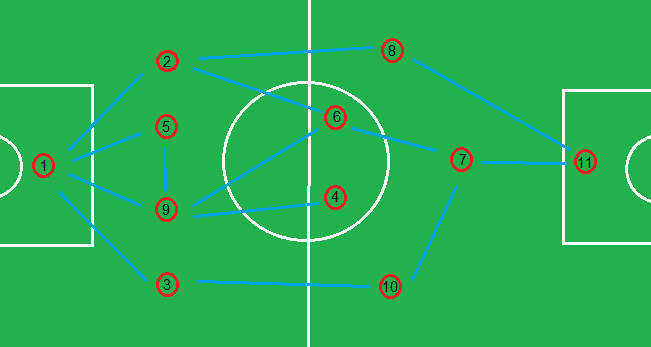
\includegraphics[width=1\textwidth]{goal-baran.png}
با توجه به این، با سه بار پاس دادن (1 به 2 و ۲ به ۸ و ۸ به ۱۱) می توان به گل رسید. یعنی در ۲۴ دقیقه. پس درکل سه گل می تواند به ثمر رساند(بازی ۹۰ دقیقه است).

\newpage
\section{فوتبال}


در مسابقات ربات‌های فوتبالیست هر تیم دو ربات دارد، دروازه‌بان و فوروارد. هاشم که خیلی علاقه دارد اطلاعات ربات ها را داشته باشد، برای ربات‌ها بلوتوث نصب کرده و اسم، مختصات افقی و عمودی ربات در زمین و فاصله توپ از ربات را برای کامپیوتر ارسال می‌کند. فرمت داده ها به صورت زیر است:\\
\begin{tcolorbox}[boxrule=0pt]
	\begin{latin}
  	  \large{
  	  	@\#forward,x=123,y=25,distance=34\#@
		}
	\end{latin}
\end{tcolorbox}
بلوتوث داده‌ها را کاراکتر به کاراکتر ارسال می‌کند و ممکن است برخی داده‌ها سالم به کامپیوتر نرسند و نویز گیرند. همچنین هر دو ربات keeper و forward هر ۱۰۰ میلی ثانیه یک دنباله داده ارسال می‌کنند.\\
هاشم میخواهد بفهمد ربات مهاجم (forward) چند گل به ثمر رسانده است و در این کار از شما کمک می‌خواهد.\\
هر گل به این صورت است که ابتدا توپ در دهانه ربات قرار گرفته و فاصله آن از ۱۰ سانتی متر کمتر می‌شود، سپس ربات شوت می‌کند و فاصله توپ به صورت صعودی زیاد می‌شود و در نهایت توپ در دروازه قرار می‌گیرد یعنی فاصله توپ حداکثر ۱۰ سانتی متر کمتر از فاصله ربات تا دروازه می‌شود. دروازه در مختصات (0,0) قرار دارد. توجه کنید اگر مسیر توپ ناگهان غیر صعودی شود شوت ناموفق است.\\
همچنین اگر حداقل ۲۰۰ کاراکتر نامعتبر متوالی خوانده شود، از آنجا به بعد تمام داده‌ها نامعتبر هستند.\\


\textbf{ورودی}\\\\
یک رشته (String) از داده‌هایی که کامپیوتر دریافت کرده در یک خط داده می‌شود. فاصله‌ها و مختصات ها اعداد حسابی هستند.\\


\textbf{خروجی}\\\\
در تنها خط خروجی تعداد گل‌هایی که فوروارد به ثمر رسانده را چاپ کنید.\\

\inputsample{
\seqsplit{
@\#forward,x=95,y=27,distance=2\#@@\#forward,x=95,y=27,distance=10\#@@\#forward,x=95,y=27,distance=18\#@@\#forward,x=95,y=27,distance=26\#@@\#forward,x=95,y=27,distance=34\#@@\#forward,x=95,y=27,distance=42\#@@\#forward,x=95,y=27,distance=50\#@@\#forward,x=95,y=27,distance=58\#@@\#forward,x=95,y=27,distance=66\#@@\#forward,x=95,y=27,distance=74\#@@\#forward,x=95,y=27,distance=82\#@@\#forward,x=95,y=27,distance=90\#@}}
می توانید ورودی را به صورت فایل از لینک دریافت کنید.  \href{https://drive.google.com/open?id=192_0wmI5WrASVv5EUhjtTE9ZM8wBzzBn}{(لینک)}
\outputsample{
1
}


\newpage
\section{تبانی}


علی و محمدحسین سرمربی دو تیم فوتبال هستند. این دو نفر با وجود این که در دو تیم مختلف هستند، از گذشته با یکدیگر آشنایی نزدیکی دارند و به صورت کاملاً غیرورزشی، یکی از آن‌ها با دیگری توافق کرده تا اطلاعات محرمانه تیم و تاکتیک‌های آن را از طریق پیام‌هایی به سرمربی حریف که دوست اوست برساند. برای این که صاحبان باشگاه از این موضوع مطلع نشوند، آن‌ها قرارداد کرده‌اند که اطلاعات را رمز کنند و سپس از طریق مجموعه‌ای از دستورات که در رشته تغییر ایجاد می‌کنند، این اطلاعات رمزگشایی خواهند شد. از آنجایی که این دو مربی سواد کافی (!) برای انجام این کار را ندارند و در دانشگاه برای تقویت زبان انگلیسی و یادگرفتن این زبان به «تدریس» !!! مشغول هستند و در اطلاعات رمزنگاری شده از زبان انگلیسی استفاده شده، برای این کار از شما کمک خواسته‌اند تا کمک کنید آن‌ها به خواسته غیرورزشی خود برسند!\\
برای این کار در ابتدا به شما یک رشته (String) و تعدادی دستور داده می‌شود. در هر مرحله، شما باید با توجه به دستور تغییراتی روی این رشته اعمال کنید و بعد از انجام هر دستور (به جز دستور پایان برنامه) رشته را دوباره چاپ کنید.\\\\
پیش از بررسی دستورات، به خطاهایی که باید آن‌ها را چاپ کنید توجه نمایید:\\\\
منظور از پیغام خطای مناسب در تمامی دستورات زیر، عبارت 
\\\lr{"CANNOT~PERFORM THE COMMAND SUCCESSFULLY"}
است. نیاز به هیچ پیام اضافه‌ای در مورد این که در کدام دستور این اتفاق افتاده و… نیست و اگر هر کدام از شرایطی که باعث اجرای ناصحیح دستورات می‌شود و در بالا ذکر شده رخ بدهد، تنها همین عبارت را باید در یک خط چاپ کرده و به خط بعدی بروید.\\\\
تنها خطای متفاوت با این خطاها، وقتی است که دستوری وارد شود که جزو هیچ کدام از این دستورات بالا نباشد. در آن صورت باید عبارت 
\lr{"THE COMMAND IS INVALID"}
 در یک خط نوشته شده و به خط بعد برود. توجه کنید که فاصله (اسپیس) اضافی در ابتدا وانتهای دستور اهمیتی ندارد و دستور همچنان صحیح است؛ یعنی 
\lr{"\texttt{\char32}\texttt{\char32}end\texttt{\char32}\texttt{\char32}"}
  با "end" فرقی ندارد اما تعداد اسپیس‌های ما بین بخش‌های دستورات باید دقیقاً به همین فرمتی که در بالا برای هر دستور نوشته شده‌اند باشد (هیچ‌گاه بیش از یک فاصله بین پارامترهای دستورات نیست). همچنین در انتهای دستور نیز هیچ عبارت اضافه‌ای نباید باشد؛ یعنی مثلاً دستور 
\lr{"delete abc -f aaaa"}
   دستوری نامعتبر محسوب می‌شود.
\\\\
دستوراتی که داریم:\\\\
\begin{tcolorbox}[boxrule=0pt]
	\begin{latin}
  	  \large{
  	  	mul
		}
	\end{latin}
\end{tcolorbox}
این دستور، بدین صورت عمل می‌کند که در رشته‌ای که در اختیار داریم، اولین دو عدد که با یک یا چندین حرف یا علامت جدا شده باشند را پیدا کرده، آن دو را در هم ضرب کرده و سپس این دو عدد و حروف بینشان را حذف کرده و عدد حاصل‌ضرب را جایگزین می‌کند.\\
\begin{tcolorbox}[boxrule=0pt]
	\begin{latin}
  	  \large{
  	  	abc-4abcdef8ads8ds
		}
	\end{latin}
\end{tcolorbox}
حاصل به صورت:\\
\begin{tcolorbox}[boxrule=0pt]
	\begin{latin}
  	  \large{
  	  	abc-32ads8ds
		}
	\end{latin}
\end{tcolorbox}
خواهد بود.\\\\
توجه کنید که اعداد می‌توانند منفی هم باشند. با این وجود اعداد اعشاری نداریم و اولین دو یا چند بار علامت منفی پشت سرهم نیز نخواهیم داشت.\\\\
در صورتی که هیچ عبارتی با فرمت ذکر شده در رشته پیدا نشود، پیغام خطای مناسب چاپ خواهد شد.\\
\noindent\rule[0.5ex]{\linewidth}{1pt}\\
\begin{tcolorbox}[boxrule=0pt]
	\begin{latin}
  	  \large{
  	  	add
		}
	\end{latin}
\end{tcolorbox}
این دستور کاملاً مشابه دستور mul است با این تفاوت که به جای ضرب عمل جمع را انجام می‌دهد.\\\\
به عنوان مثال در صورت اجرای این دستور روی رشته\\
\begin{tcolorbox}[boxrule=0pt]
	\begin{latin}
  	  \large{
  	  	abc-4abcdef8ads8ds
		}
	\end{latin}
\end{tcolorbox}
حاصل به صورت:
\begin{tcolorbox}[boxrule=0pt]
	\begin{latin}
  	  \large{
  	  	abc4ads8ds
		}
	\end{latin}
\end{tcolorbox}
خواهد بود.\\\\
توجه کنید که اعداد می‌توانند منفی هم باشند. با این وجود اعداد اعشاری نداریم و دو یا چند بار علامت منفی پشت سرهم نیز نخواهیم داشت.\\\\
در صورتی که هیچ عبارتی با فرمت ذکر شده در رشته پیدا نشود، پیغام خطای مناسب چاپ خواهد شد.\\
\noindent\rule[0.5ex]{\linewidth}{1pt}\\
\begin{tcolorbox}[boxrule=0pt]
	\begin{latin}
  	  \large{
  	  	sub
		}
	\end{latin}
\end{tcolorbox}
این دستور نیز کاملاً مشابه دستور mul است با این تفاوت که به جای ضرب عمل تفریق را انجام می‌دهد. بدین صورت که عددی که اول آمده (در سمت چپ) را منهای عددی که دوم آمده (در سمت راست) می‌کند؛ به عبارت دیگر عدد دوم را از عدد اول کم می‌کند.\\\\
به عنوان مثال در صورت اجرای این دستور روی رشته
\begin{tcolorbox}[boxrule=0pt]
	\begin{latin}
  	  \large{
		abc-4abcdef8ads8ds
		}
	\end{latin}
\end{tcolorbox}
حاصل به صورت:
\begin{tcolorbox}[boxrule=0pt]
	\begin{latin}
  	  \large{
  	  	abc-12ads8ds
		}
	\end{latin}
\end{tcolorbox}
خواهد بود.\\\\
توجه کنید که اعداد می‌توانند منفی هم باشند. با این وجود اعداد اعشاری نداریم و دو یا چند بار علامت منفی پشت سرهم نیز نخواهیم داشت.\\\\
در صورتی که هیچ عبارتی با فرمت ذکر شده در رشته پیدا نشود، پیغام خطای مناسب چاپ خواهد شد.\\
\noindent\rule[0.5ex]{\linewidth}{1pt}\\
\begin{tcolorbox}[boxrule=0pt]
	\begin{latin}
  	  \large{
  	  	sum [n] [-f or -b]
		}
	\end{latin}
\end{tcolorbox}
این دستور بدین صورت است که در ابتدا کلمه کلیدی sum آمده، سپس با یک فاصله یک عدد (n) می‌آید و پس از آن با یک فاصله 
\lr{"-f"}
 یا 
 \lr{"-b"} 
 نوشته می‌شود. عملکرد این دستور بدین صورت است که از از انتها یا ابتدای رشته، به دنبال n  عدد می‌گردد. (برای 
\lr{"-f"} 
  از انتها و برای 
\lr{"-b"}
  از ابتدا). اگر n عدد پیدا نکرد، پیام خطای مناسب چاپ می‌شود. در غیر این صورت، این n عدد را با هم جمع کرده و با فرمت
\lr{"S[sum]S"} 
 در انتهای رشته می‌نویسد.\\\\
به عنوان مثال رشته زیر را در نظر بگیرید:
\begin{tcolorbox}[boxrule=0pt]
	\begin{latin}
  	  \large{
		a1b2c3d4e5f6g
		}
	\end{latin}
\end{tcolorbox}
در صورت اجرای دستور:
\begin{tcolorbox}[boxrule=0pt]
	\begin{latin}
  	  \large{
  	  	sum 3 -b
		}
	\end{latin}
\end{tcolorbox}
حاصل به صورت زیر خواهد بود:
\begin{tcolorbox}[boxrule=0pt]
	\begin{latin}
  	  \large{
  	  	a1b2c3d4e5f6gS6S
		}
	\end{latin}
\end{tcolorbox}
و در صورتی که روی همان رشته اول دستور زیر را اجرا می‌کردیم:
\begin{tcolorbox}[boxrule=0pt]
	\begin{latin}
  	  \large{
  	  	sum 3 -f
		}
	\end{latin}
\end{tcolorbox}
حاصل به صورت
\begin{tcolorbox}[boxrule=0pt]
	\begin{latin}
  	  \large{
  	  	a1b2c3d4e5f6gS15S
		}
	\end{latin}
\end{tcolorbox}
در‌می‌آید.\\\\
\noindent\rule[0.5ex]{\linewidth}{1pt}
\begin{tcolorbox}[boxrule=0pt]
	\begin{latin}
  	  \large{
  	  	gcd [n] [-f or -b]
		}
	\end{latin}
\end{tcolorbox}
این دستور تا حد زیادی مشابه دستور sum است. با این تفاوت که به جای محاسبه جمع اعداد، ب.م.م آن‌ها را محاسبه می‌کند. این دستور بدین صورت است که در ابتدا کلمه کلیدی gcd آمده، سپس با یک فاصله یک عدد (n) می‌آید و پس از آن با یک فاصله 
\lr{"-f"} 
یا
\lr{"-b"} 
نوشته می‌شود. عملکرد این دستور بدین صورت است که از انتها یا ابتدای رشته، به دنبال n  عدد می‌گردد. (برای 
\lr{"-f"} 
 از انتها و برای 
\lr{"-b"}
  از ابتدا). اگر n عدد پیدا نکرد، پیام خطای مناسب چاپ می‌شود. در غیر این صورت، ب.م.م این n عدد را محاسبه می‌کند و با فرمت
\lr{"G[gcd]G"}
  در انتهای رشته می‌نویسد.\\\\
به عنوان مثال رشته زیر را در نظر بگیرید:
\begin{tcolorbox}[boxrule=0pt]
	\begin{latin}
  	  \large{
		a12b18c24d10e15f25z
		}
	\end{latin}
\end{tcolorbox}
در صورت اجرای دستور:
\begin{tcolorbox}[boxrule=0pt]
	\begin{latin}
  	  \large{
  	  	gcd 3 -b
		}
	\end{latin}
\end{tcolorbox}
حاصل به صورت زیر خواهد بود:
\begin{tcolorbox}[boxrule=0pt]
	\begin{latin}
  	  \large{
  	  	a12b18c24d10e15f25zG6G
		}
	\end{latin}
\end{tcolorbox}
و در صورتی که روی همان رشته اول دستور زیر را اجرا می‌کردیم:
\begin{tcolorbox}[boxrule=0pt]
	\begin{latin}
  	  \large{
  	  	gcd 3 -f
		}
	\end{latin}
\end{tcolorbox}
حاصل به صورت
\begin{tcolorbox}[boxrule=0pt]
	\begin{latin}
  	  \large{
  	  	a12b18c24d10e15f25zG5G
		}
	\end{latin}
\end{tcolorbox}
در‌می‌آید.\\\\
\noindent\rule[0.5ex]{\linewidth}{1pt}
\begin{tcolorbox}[boxrule=0pt]
	\begin{latin}
  	  \large{
  	  	replace [str1] [str2] [n]
		}
	\end{latin}
\end{tcolorbox}
این دستور بدین صورت است که باید در رشته اصلی که در اختیار داریم، رشته str1 را پیدا کرده و رشته str2 را جایگزین کنیم. عدد n که در انتها می‌آید، مشخص می‌کند که این کار چند بار باید انجام شود. توجه کنید که وقتی مثلاً n=2 است، بعد از این که برای بار اول str2 را جایگزین str1 کردیم، باید دوباره از ابتدا به جست و جو برای str1 در رشته اصلی بپردازید؛ یعنی ممکن است در اثر جایگزینی str2 به جای str1، خود عبارت str1 به شکل دیگری در اثر این جایگزینی ایجاد شود که باید آن هم در نظر گرفته بشود.\\\\
در صورتی که امکان انجام این عمل به تعداد n بار وجود نداشت (یعنی n بار str1 پیدا نشد)، به همان تعدادی که پیدا شده اعمال انجام می‌شوند و نیازی به چاپ کردن پیام خطایی در صورت بروز این مشکل نیست.\\\\
تضمین می‌شود که n عددی نامنفی است.\\\\
مثال:\\
رشته اصلی:\\
\begin{tcolorbox}[boxrule=0pt]
	\begin{latin}
  	  \large{
		abcdddabcdddabcddd
		}
	\end{latin}
\end{tcolorbox}
دستور:
\begin{tcolorbox}[boxrule=0pt]
	\begin{latin}
  	  \large{
  	  	replace abc xyz 2
		}
	\end{latin}
\end{tcolorbox}
نتیجه:
\begin{tcolorbox}[boxrule=0pt]
	\begin{latin}
  	  \large{
  	  	xyzdddxyzdddabcddd
		}
	\end{latin}
\end{tcolorbox}
\noindent\rule[0.5ex]{\linewidth}{1pt}
\begin{tcolorbox}[boxrule=0pt]
	\begin{latin}
  	  \large{
  	  	count\_entail [str]
		}
	\end{latin}
\end{tcolorbox}
این دستور، تعداد تمامی دفعاتی که رشته str در رشته اصلی ظاهر شده را شمرده و در انتهای رشته اصلی، عبارتی با فرمت C[count]C اضافه می‌کند. توجه کنید که این دستور، باید همپوشانی (Overlap) شدن عبارات را هم در نظر گرفته و در شمارش به حساب بیاورد. برای واضح‌تر شدن این موضوع رشته اصلی زیر را در نظر بگیرید:
\begin{tcolorbox}[boxrule=0pt]
	\begin{latin}
  	  \large{
		abcabca
		}
	\end{latin}
\end{tcolorbox}
در صورت اجرای دستور:
\begin{tcolorbox}[boxrule=0pt]
	\begin{latin}
  	  \large{
  	  	count\_entail abca
		}
	\end{latin}
\end{tcolorbox}
باید رشته نهایی به صورت زیر بشود:
\begin{tcolorbox}[boxrule=0pt]
	\begin{latin}
  	  \large{
  	  	abcabcaC2C
		}
	\end{latin}
\end{tcolorbox}
در صورتی که رشته str کلاً در رشته اصلی پیدا نشود، نیازی به تغییر در رشته اصلی و اضافه کردن عبارت به انتهای آن نیست و باید پیام خطای مناسب چاپ شود.\\\\
\noindent\rule[0.5ex]{\linewidth}{1pt}
\begin{tcolorbox}[boxrule=0pt]
	\begin{latin}
  	  \large{
  	  	insert [str] [count - optional]
		}
	\end{latin}
\end{tcolorbox}
این دستور به دو شکل می‌آید. در حالت اول کلمه insert و یک عبارت بعد از آن می‌آید. در این صورت در انتهای رشته اصلی باید عبارت مد نظر اضافه شود.\\
در فرمت دوم، بعد از رشته str یک عدد هم می‌آید که اندیس یک نقطه مشخص در رشته اصلی است و باید str بعد از آن اندیس به رشته اصلی اضافه شود. ابتدای رشته و قبل از تمامی حروف با اندیس 0 مشخص می‌شود. در صورتی که این عدد از کل طول رشته بزرگ‌تر باشد، هیچ تغییری در رشته انجام نشده و پیام خطای مناسب نوشته خواهد شد.\\
به عنوان مثال رشته اصلی زیر را در نظر بگیرید:\\
\begin{tcolorbox}[boxrule=0pt]
	\begin{latin}
  	  \large{
		ad
		}
	\end{latin}
\end{tcolorbox}
در صورت اجرای دستور:
\begin{tcolorbox}[boxrule=0pt]
	\begin{latin}
  	  \large{
  	  	insert bc 1
		}
	\end{latin}
\end{tcolorbox}
نتیجه به صورت:
\begin{tcolorbox}[boxrule=0pt]
	\begin{latin}
  	  \large{
  	  	abcd
		}
	\end{latin}
\end{tcolorbox}
در صورت اجرای دستور:
\begin{tcolorbox}[boxrule=0pt]
	\begin{latin}
  	  \large{
  	  	insert bc
		}
	\end{latin}
\end{tcolorbox}
مستقل از دستور قبلی، نتیجه به صورت:
\begin{tcolorbox}[boxrule=0pt]
	\begin{latin}
  	  \large{
  	  	adbc
		}
	\end{latin}
\end{tcolorbox}
در صورت اجرای دستور:
\begin{tcolorbox}[boxrule=0pt]
	\begin{latin}
  	  \large{
  	  	insert bc 0
		}
	\end{latin}
\end{tcolorbox}
مستقل از دستور قبلی، نتیجه به صورت:
\begin{tcolorbox}[boxrule=0pt]
	\begin{latin}
  	  \large{
  	  	bcad
		}
	\end{latin}
\end{tcolorbox}
خواهد بود.\\
\noindent\rule[0.5ex]{\linewidth}{1pt}
\begin{tcolorbox}[boxrule=0pt]
	\begin{latin}
  	  \large{
  	  	delete [str] [-f -optional]
		}
	\end{latin}
\end{tcolorbox}
این دستور نیز به دو شکل می آید. در شکل اول کلمه delete و پس از آن یک رشته str می آید. در این صورت، باید در رشته اصلی، به دنبال اولین str بگردید و اولین دفعه ای که این رشته درون رشته اصلی ظاهر شده را حذف نمایید. در شکل دوم بعد از str با یک فاصله عبارت 
\lr{"-f"}
 هم نوشته می شود. در این صورت باید در رشته اصلی به دنبال str بگردید و آخرین دفعه ای که ظاهر شده را حذف کنید. در صورتی که رشته مورد نظر کلا وجود نداشت، باید پیام خطای مناسب را چاپ کنید.\\
به عنوان مثال رشته اصلی زیر را در نظر بگیرید:\\
\begin{tcolorbox}[boxrule=0pt]
	\begin{latin}
  	  \large{
		zabczabcz
		}
	\end{latin}
\end{tcolorbox}
در صورت اجرای دستور:
\begin{tcolorbox}[boxrule=0pt]
	\begin{latin}
  	  \large{
  	  	delete abc
		}
	\end{latin}
\end{tcolorbox}
نتیجه به صورت زیر خواهد بود:
\begin{tcolorbox}[boxrule=0pt]
	\begin{latin}
  	  \large{
  	  	zzabcz
		}
	\end{latin}
\end{tcolorbox}
و در صورت اجرای دستور:
\begin{tcolorbox}[boxrule=0pt]
	\begin{latin}
  	  \large{
  	  	delete abc -f
		}
	\end{latin}
\end{tcolorbox}
نتیجه به صورت زیر خواهد بود:
\begin{tcolorbox}[boxrule=0pt]
	\begin{latin}
  	  \large{
  	  	zabczz
		}
	\end{latin}
\end{tcolorbox}
\noindent\rule[0.5ex]{\linewidth}{1pt}
\begin{tcolorbox}[boxrule=0pt]
	\begin{latin}
  	  \large{
  	  	print
		}
	\end{latin}
\end{tcolorbox}
همان طور که مشخص است، این دستور رشته را به همان شکلی که هست، چاپ خواهد کرد.\\\\
\noindent\rule[0.5ex]{\linewidth}{1pt}
\begin{tcolorbox}[boxrule=0pt]
	\begin{latin}
  	  \large{
  	  	end
		}
	\end{latin}
\end{tcolorbox}
به اجرای برنامه پایان می‌دهد. پس از این دستور، باید عبارت
\lr{END OF PROGRAM}
  در خط جدید چاپ شده و برنامه به اتمام برسد.\\\\
در تمامی دستورات بالا به جز مواردی که ذکر شده، اعداد همگی نامنفی خواهند بود و نیازی به انجام هیچ نوع بررسی در این موارد ندارید.\\

\textbf{ورودی}\\\\
در خط اول به شما یک رشته اصلی اولیه داده می‌شود. سپس در خطوط بعدی، تعدادی دستور وارد می‌شود که بسته به توضیحات بالا تغییراتی را در آن رشته اعمال می‌کنند. توجه کنید که تعداد دستورات مشخص نیست وانتهای آن‌ها با دستور "end" مشخص می‌شود که پس از آن، برنامه به پایان می‌رسد.\\
در مورد اعدادی که در قسمت‌های مختلف سوال استفاده می‌شوند، تضمین می‌شود که محدوده اعداد از "int" فراتر نخواهد رفت.\\
لازم به ذکر است که درون رشته اصلی فاصله (اسپیس) نداریم و در طول مراحل مختلف نیزفاصله درون آن ایجاد نخواهد شد.\\


\textbf{خروجی}\\\\
بسته به نوع دستور و توضیحاتی که در بالا ذکر شده، باید در هر مرحله خروجی مخصوص داده شود. در صورتی که دستور اشتباه باشد 
\lr{"THE COMMAND IS INVALID"} 
- در صورتی که در حین اجرای دستور بر اساس توضیحات بالا مشکلی ایجاد بشود 
\\\lr{"CANNOT PERFORM THE COMMAND SUCCESSFULLY"} 
و در پایان برنامه هم عبارت
\lr{"END OF PROGRAM"}
 نوشته خواهد شد. به جز برای دستور پایان، برای سایر دستورات باید بعد در صورت اجرای موفقیت‌آمیز دستور، شکل جدید رشته نوشته بشود.\\


\inputsample{
\seqsplit{
-1o-1RingToRuleThemAll-1o-1RingToFindThem1o1RingToBringThemAllAndInTheDarknessBindThem\\}
\texttt{\char32}\texttt{\char32}mul\\
replace 1 One 1\\
mul\\
replace 1 One 1\\
mult\\
mul\\
replace 1 One 1\\
mul\\
replace 1 One 1\\
replacee Ring Nazg 4\\
replace Ring Nazg 4\\
replace ToRule Durbat 1\\
replace ToBring Thrakat 1\\
replace InTheDarkness BurzumIshi 1\\
replace Bind Krimp 1\\
delete To -f -f\\
delete To -f\\
replace ThemAll uluk 2\\
replace Them atul 2\\
replace And Agh 1\\
replace Find Gimb 10\\
replace One Ash 2\\
replace One Ash 2\\
insert Mordor\\
insert \_ 72\\
insert 4oo4oo22oo\\
gcd 2 -b\\
gcd 4 -f\\
sum 2 -b\\
count\_entail oo\\
delete 4oo4oo22ooG4GG2GS8SC3C\\
print\\
end
}
می توانید ورودی را به صورت فایل از لینک دریافت کنید.  \href{https://drive.google.com/open?id=1z-Un8Qde0elQkFgT8rxtkGRZRjN149hz}{(لینک)}
\outputsample{
\seqsplit{
1RingToRuleThemAll-1o-1RingToFindThem1o1RingToBringThemAllAndInTheDarknessBindThem\\
OneRingToRuleThemAll-1o-1RingToFindThem1o1RingToBringThemAllAndInTheDarknessBindThem\\
OneRingToRuleThemAll1RingToFindThem1o1RingToBringThemAllAndInTheDarknessBindThem\\
OneRingToRuleThemAllOneRingToFindThem1o1RingToBringThemAllAndInTheDarknessBindThem\\}
THE COMMAND IS INVALID\\
\seqsplit{
OneRingToRuleThemAllOneRingToFindThem1RingToBringThemAllAndInTheDarknessBindThem\\
OneRingToRuleThemAllOneRingToFindThemOneRingToBringThemAllAndInTheDarknessBindThem\\}
CANNOT PERFORM THE COMMAND SUCCESSFULLY\\
\seqsplit{
OneRingToRuleThemAllOneRingToFindThemOneRingToBringThemAllAndInTheDarknessBindThem\\}
THE COMMAND IS INVALID\\
\seqsplit{
OneNazgToRuleThemAllOneNazgToFindThemOneNazgToBringThemAllAndInTheDarknessBindThem\\
OneNazgDurbatThemAllOneNazgToFindThemOneNazgToBringThemAllAndInTheDarknessBindThem\\
OneNazgDurbatThemAllOneNazgToFindThemOneNazgThrakatThemAllAndInTheDarknessBindThem\\
OneNazgDurbatThemAllOneNazgToFindThemOneNazgThrakatThemAllAndBurzumIshiBindThem\\
OneNazgDurbatThemAllOneNazgToFindThemOneNazgThrakatThemAllAndBurzumIshiKrimpThem\\}
THE COMMAND IS INVALID\\
\seqsplit{
OneNazgDurbatThemAllOneNazgFindThemOneNazgThrakatThemAllAndBurzumIshiKrimpThem\\
OneNazgDurbatulukOneNazgFindThemOneNazgThrakatulukAndBurzumIshiKrimpThem\\
OneNazgDurbatulukOneNazgFindatulOneNazgThrakatulukAndBurzumIshiKrimpatul\\
OneNazgDurbatulukOneNazgFindatulOneNazgThrakatulukAghBurzumIshiKrimpatul\\
OneNazgDurbatulukOneNazgGimbatulOneNazgThrakatulukAghBurzumIshiKrimpatul\\
AshNazgDurbatulukAshNazgGimbatulOneNazgThrakatulukAghBurzumIshiKrimpatul\\
AshNazgDurbatulukAshNazgGimbatulAshNazgThrakatulukAghBurzumIshiKrimpatul\\
AshNazgDurbatulukAshNazgGimbatulAshNazgThrakatulukAghBurzumIshiKrimpatulMordor\\
AshNazgDurbatulukAshNazgGimbatulAshNazgThrakatulukAghBurzumIshiKrimpatul\_Mordor\\
AshNazgDurbatulukAshNazgGimbatulAshNazgThrakatulukAghBurzumIshiKrimpatul\_Mordor4oo4oo22oo
AshNazgDurbatulukAshNazgGimbatulAshNazgThrakatulukAghBurzumIshiKrimpatul\_Mordor4oo4oo22ooG4G\\
AshNazgDurbatulukAshNazgGimbatulAshNazgThrakatulukAghBurzumIshiKrimpatul\_Mordor4oo4oo22ooG4GG2G\\
AshNazgDurbatulukAshNazgGimbatulAshNazgThrakatulukAghBurzumIshiKrimpatul\_Mordor4oo4oo22ooG4GG2GS8S\\
AshNazgDurbatulukAshNazgGimbatulAshNazgThrakatulukAghBurzumIshiKrimpatul\_Mordor4oo4oo22ooG4GG2GS8SC3C\\
AshNazgDurbatulukAshNazgGimbatulAshNazgThrakatulukAghBurzumIshiKrimpatul\_Mordor\\
AshNazgDurbatulukAshNazgGimbatulAshNazgThrakatulukAghBurzumIshiKrimpatul\_Mordor\\}
END OF PROGRAM
}
می توانید خروجی را به صورت فایل از لینک دریافت کنید.  \href{https://drive.google.com/open?id=1xizAD0Ctv0SDGLtcc-7iAhKyuIbDXtSN}{(لینک)}
\end{document}









